\chapter{Methodology}
The software methodology used to develop this project will be described in this
chapter. Agile methodologies have been used to drive Alcaudon's development.

Agile methodologies help organizing software development life cycle. They are
focused on iterative development and adaptability. The term was coined during
the early 2000s in the \textit{Agile Manifesto}\cite{manifesto}. The manifesto
has this set of principles:

\begin{itemize}
\item Individuals and interactions over processes and tools
\item Working software over comprehensive documentation
\item Customer collaboration over contract negotiation
\item Responding to change over following a plan
\end{itemize}

The main goal of these methodologies is to improve communications between all
the stakeholders in a project. This focus on continuous communications reduces
risks and provides value since the very beginning of the project. One of the
outcomes of this iterative open process is a reduction in the costs of the
changes. This differs totally from rigid methodologies such as waterfall where
the customer is taken apart from the project until the very end, skyrocketing
the costs of change.

Agile methodologies have become popular during the last 10 years, therefore there
are many agile frameworks that follow the previously enumerated principles. The
most popular ones are:
\begin{itemize}
\item SCRUM\cite{scrum}: Framework that allows teams to develop complex
  adaptive software delivering value as soon as possible.
\item eXtreme Programming\cite{xp}: Lightweight methodology for small-medium
  sized software development teams in scenarios where requirements change often
  or are vague.
\item Kanban\cite{kanban}: Inspired by the work of Toyota during the 1940s to improve
  factory resource utilization, this lightweight methodology also minimizes the processes
  around development. It is focused on having a set of features to be done and delivering
  them as soon as possible. It is a good fit for startup teams.
\end{itemize}

Since Alcaudon's requirements were not clear from the start agile methodologies
provided the optimal framework. In particular, eXtreme Programming was chosen
due to the team's small size and the expected requirement changes.

\section{eXtreme Programming}

\begin{figure}
  \centering
  \includegraphics[width=0.6\textwidth]{xp.png}
  \caption{Extreme Programming feedback diagram\cite{xp}}
  \label{fig:xp}
\end{figure}

This methodology proposes a feedback/release cycle as shown in Figure~\ref{fig:xp} and a set of
practices\cite{xp}:

\begin{enumerate}
\item \textit{The planning game}: The scope, priority and date of releases
  should be agreed between business and technical team, adapting them in the
  face of unplanned events. Neither business nor technical parties involved have
  more weight than the other when planning next releases. This is why
  communication is one of the key principles in this methodology. In Alcaudon
  the business team was represented by the advisor, \textit{David Villa Alises},
  and the technical team by the author.
\item Small releases: Every release should be as small as possible providing the
  maximum business value. Alcaudon is released continuously, meaning that it has
  adopted Continuous Deployment\cite{cd} techniques. Every commit pushed to the
  master branch, Travis CI (footnote) launches a continuous delivery pipeline
  that runs tests, builds and publishes an usable version of Alcaudon as docker
  containers and a snapshot version of the libraries to Maven central. This
  practice allows Alcaudon's process to bring value as soon as possible.
  Moreover, it reduces risks, thus contributing to build a more efficient and
  robust system.
\item \textit{Metaphor}: A common language between different participants in the
  project should be use. This makes communication easier and therefore
  misunderstandings are reduced.
\item Simple design: As defined by\cite{xp}, a simple design follows these rules:
  \begin{enumerate}
  \item All tests pass.
  \item There is no duplicated logic.
  \item States every intention important to the programmers.
  \item Has the fewest possible classes, methods and functions.
  \end{enumerate}
  Alcaudon follows these principles. Consequently, the risks associated to
  changes are minimized.
\item Testing: In XP there is a strong bias towards writing tests for all the
  created functionalities, both unit and functional tests. This practice creates
  a stronger confidence in programmers when they need to change their code.
  Alcaudon has been tested broadly, using unit, integration and property based
  testing. Having a good testing coverage has helped to keep developing the
  system with confidence in its correctness, since this project can not be
  easily tested manually.
\item Refactoring: Given the previous principle of \textit{simple design},
  continuous design refinement via refactoring is a key concept in XP.
  Refactoring helps to keep control of complexity iterating over software
  design, reducing risks in future changes. During the development of this
  project, there have been some refactors that improved the design of certain
  modules. Following this principle has been crucial to improve the system's
  architecture.
\item Pair programming: In this methodology there is a preference towards programming
  in pairs. Different points of view can improve the final design and spot
  possible failures that otherwise would have taken longer to detect. This
  principle does not apply to Alcaudon since it is an individual project.
\item Continuous Integration: Code should be integrated and tested every few
  hours. This practice helps to avoid working too long in a big feature, making
  it harder to integrate later. Again, XP is favoring risk reduction with this
  set of practices. As described before, Alcaudon uses Travis CI as continuous
  integration server, for every commit to master the project is built and
  tested.
\item On-site customer: XP accentuates the importance of communications. A
  domain expert, i.e. an user, should be available to answer questions about the
  business and set small scale priorities. Having this person accessible, saves
  time when developers are not familiar with some details about the domain, therefore
  reducing risks.
\item Coding standards: Every project should have coding standards so the
  differences in style among the code written by the team are minimized. An
  example could be a code linter, so if there is a deviation in the defined
  style the programmer will be warned. There are more sophisticated tools to
  define standards, such as code quality measurements tools. These metrics can
  be added in the continuous integration pipeline. if the added code does not
  comply with them, the build is marked as failed. This project uses a code
  linter and advanced compiler warnings (such as unused code, deprecated APIs,
  etc), therefore the coding style is uniform.
\end{enumerate}

\subsection{eXtreme Programming applied to this project}

This section describes the different releases done during the development of
Alcaudon. As it has been stated before, Continuous Deployment has been
implemented, so there has been a production ready release after every code
change. For simplicity this section will describe release cycles with blocks of
features.

\subsubsection{Release 1: State of the art analysis}
\begin{itemize}
\item \textit{Agreed goal}: Distributed data processing systems State of the art analysis.
  \item \textit{Deliverable}: Document describing existing solutions in the
    distributed data processing space as well as recent developments from
    different related conferences such as, VLDB, SIGMOD and OSDI.
\end{itemize}

\subsubsection{Release 2: Technology selection}
\begin{itemize}
\item \textit{Agreed goal}: Given the findings from the previous week,
  investigate suitable technologies to implement a distributed data processing
  system.
\item \textit{Deliverable}: After some investigation and tests two languages
  were chosen, Erlang and Scala. Both implement the actor model. Erlang has been
  proven to be production ready, but according to TIOBE\cite{tiobe} its usage is
  not ample. On the other hand, Scala seems to be quite popular among the data
  processing community. After some discussion with business stakeholders, Scala
  was chosen due to its inter-operability with Java and notoriety among
  developers.
\end{itemize}

\subsubsection{Release 3: Computation, timer, source and sink API definitions}
\begin{itemize}
\item \textit{Agreed goal}: Define the public interface that customers will use
  to implement their computations and timers as well as sources and sinks.
\item \textit{Deliverable}: During this release cycle, communication between the
  different participants in the project was quite productive. A first proposal
  was sent to the domain expert, the advisor in this project. This first version
  did not take into account certain details that were key to the project. Given
  the early feedback, it was possible to react quickly and present a new
  computation API that contained less details about the implementation,
  providing a better abstraction.
\end{itemize}

\subsubsection{Release 4: Dataflow builder development}
\begin{itemize}
\item \textit{Agreed goal}: Develop a first dataflow builder version where the
  user can define a dataflow topology.
\item \textit{Deliverable}: During this week an usable dataflow builder was
  delivered. Alcaudon users were able to build their own computation topologies.
  This allowed to start testing how usable the interface was and with the given
  feedback improve the initial designs.
\end{itemize}

\subsubsection{Release 5: First computation execution engine version development}
\begin{itemize}
\item \textit{Agreed goal}: Implement the first version for the computation
  execution engine.
\item \textit{Deliverable}: Since Dataflow builder was developed during the previous
  release, the next natural step was to implement the computation executor.
  During this release a simplified engine version was released, making possible
  to test simple computations.
\end{itemize}

\subsubsection{Release 6: Computation execution guarantees development}
\begin{itemize}
\item \textit{Agreed goal}: One of the Alcaudon goals is to be fault-tolerant.
  During this release cycle it was agreed to implement the means to provide
  fault-tolerant computation executions.
\item \textit{Deliverable}: The outcome of this release cycle was fully tested
  computation engine that complies with the fault-tolerant agreed requirements.
\end{itemize}

\subsubsection{Release 7: Timer execution engine development}
\begin{itemize}
\item \textit{Agreed goal}: Alcaudon works with unbounded data-sets, hence a way to
  emit partial results should be provided. During this release cycle was agreed to implement
  fixed timers as well as watermark based timers.
\item \textit{Deliverable}: During this release cycle the feedback from the advisor
  was
\end{itemize}

\subsubsection{Release 8: Generic serialization library development}
\begin{itemize}
\item \textit{Agreed goal}: Define the public interface that customers will
  use to implement their computations.
\item \textit{Deliverable}: During this release cycle the feedback from the advisor
  was
\end{itemize}

\subsubsection{Release 9: Distributed architecture}
\begin{itemize}
\item \textit{Agreed goal}: Define the public interface that customers will
  use to implement their computations.
\item \textit{Deliverable}: During this release cycle the feedback from the advisor
  was
\end{itemize}

\subsubsection{Release 10: Distributed architecture}
\begin{itemize}
\item \textit{Agreed goal}: Define the public interface that customers will
  use to implement their computations.
\item \textit{Deliverable}: During this release cycle the feedback from the advisor
  was
\end{itemize}

\subsection{Technology choices}
\lipsum

%% \newpage

%% \begin{landscape}
%% \begin{figure}
%%   \centering
%%   \includegraphics[width=1\textwidth]{mindmap.png}
%%   \caption{caption}
%%   \label{fig:label}
%%  \end{figure}
%%     %% \includegraphics[width=0.6\textwidth]{mindmap.png}
%%     %% \caption{Property profile of the diverse library compared to the compound pool.}
%%     %% \label{fig:PropProf}
%% \end{landscape}
